\documentclass{standalone}
\usepackage[dvipsnames]{xcolor}
\usepackage{upgreek}
\usepackage{filecontents,pgfplots}
\usetikzlibrary{patterns}
\begin{document}
\pgfplotsset{
    standard/.style={
  axis x line*=bottom,
  axis y line*=right,
        axis x line shift=0.1,
        enlargelimits=false
    }
}
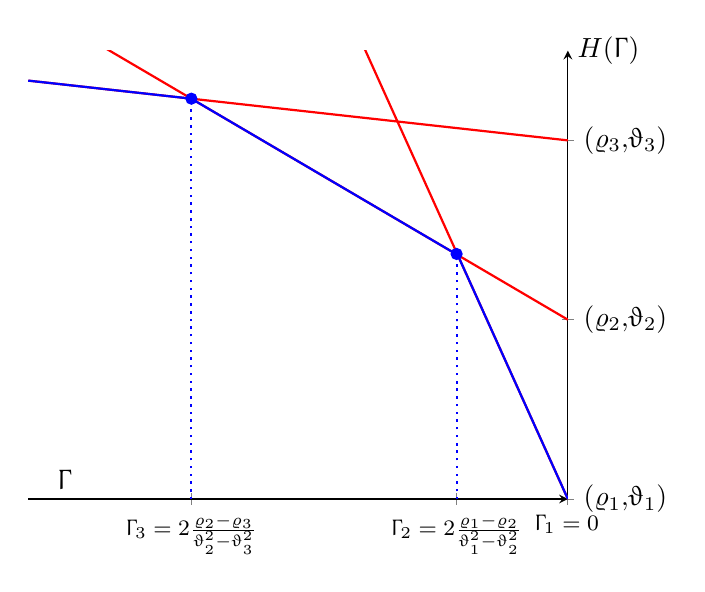
\begin{tikzpicture}[scale=1]
\begin{axis}[xmin=-5,xmax=0,ymin=0,ymax=3.75,
  %axis lines=center,
      axis y line=right, 
    axis x line=middle,
      xlabel={$\Upgamma$}, 
    ylabel={$H(\Upgamma)$} , 
    ylabel style={rotate=-90},
            xtick={-3.4883,-1.0309,-0.01},
            xticklabels={{\footnotesize${\Upgamma}_{3}=2\frac{\varrho_2-\varrho_3}{\upvartheta_2^2-\upvartheta_3^2}$},{\footnotesize${\Upgamma}_{2}=2\frac{\varrho_1-\varrho_2}{\upvartheta_1^2-\upvartheta_2^2}$},{\footnotesize${\Upgamma}_1=0$}},
        ytick={0,1.5,3},
        yticklabels={$(\varrho_1{,}\upvartheta_1)$,$(\varrho_2{,}\upvartheta_2)$,$(\varrho_3{,}\upvartheta_3)$},
            every axis y label/.append style={at=(ticklabel* cs:1)},
            every axis x label/.append style={at=(ticklabel* cs:.1)},
            y tick label style={right},
                    ]
         %\addplot[white,pattern color = red, pattern = north east lines,opacity=.5] coordinates {(1,0) (2 ,-1)  (3,-1.5) (3,3) (-1, 4) (1,0)};
    \addplot[thick, red,domain=-5:0, samples=100]{3-.1*x};
\addplot [thick,red,domain=-5:0, samples=100]{0-2*x};

  \addplot [thick,red,domain=-5:0, samples=100]{1.5-.53*x};
    
    \addplot [thick,blue,dotted,domain=0:2.05, samples=100](-1.0309,x);
    \addplot [thick,blue,dotted,domain=0:3.34883, samples=100](-3.4883,x);
    
    
 \addplot [thick,blue,domain=-5:-3.4883, samples=100]{3-0.1*x};
 \addplot [thick,blue,domain=-3.4883:-1.0309, samples=100]{1.5-.53*x};
 \addplot [thick,blue,domain=-1.0309:0, samples=100]{0-2*x};

    
%\addplot[blue,thick] (cs:(0,0.5))  (cs:(-1.0309,2.05));

\addplot[only marks, mark=*, blue] table {
   -3.4883 3.34883
  };
  \addplot[only marks, mark=*, blue] table {
  -1.0309  2.05
  };
  \addplot[only marks, mark=diamond*, blue] table {
  2  -1
  };
  \node [rotate=48] at (axis cs:  .7,  .59) {$$};
\end{axis}
\end{tikzpicture}

\end{document}